\documentclass{article}
\usepackage[supp]{naturetex}

\begin{document}

\maketitle

\beginsupplement

% *** SUPPLEMENTARY METHODS ***
\newpage
\section*{Supplementary Figures}

\begin{figure}[h]
	\begin{center}
		
\includegraphics[width=\textwidth]{supfig1}
	\end{center}
	\caption{\textbf{\lipsum[30][1]} \lipsum[30][2]}
	\label{sup.fig:my_sup_plot1}
\end{figure}

\clearpage
\begin{figure}[h]
	\begin{center}
		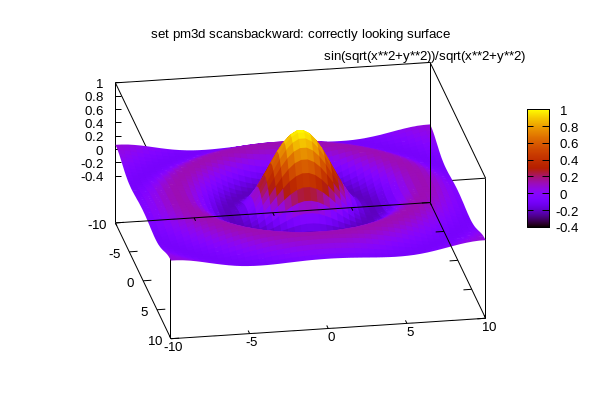
\includegraphics[width=\textwidth]{supfig2}
	\end{center}
	\caption{\textbf{\lipsum[30][3]} \lipsum[30][4]}
	\label{sup.fig:my_sup_plot2}
\end{figure}

% *** SUPPLEMENTARY METHODS ***
\newpage
\section*{Supplementary Methods}

\subsection*{\lipsum[45][1]}
\lipsum[40][1]
\cite{pearson1901liii}
\lipsum[40][2]
\ref{fig:my_plot1} and \ref{fig:my_plot2}.
\lipsum[40][3-100]

\subsection*{\lipsum[45][2]}
\lipsum[41][1-3]
\cite{chopra2005learning}
\lipsum[41][4-100]
\ref{sup.fig:my_sup_plot1}

\lipsum[51][1]
\cite{hermans2017defense}
\lipsum[51][2-100]
\ref{sup.fig:my_sup_plot2} and \ref{sup.fig:my_sup_plot3}

\begin{figure}[h]
	\makebox[\textwidth]{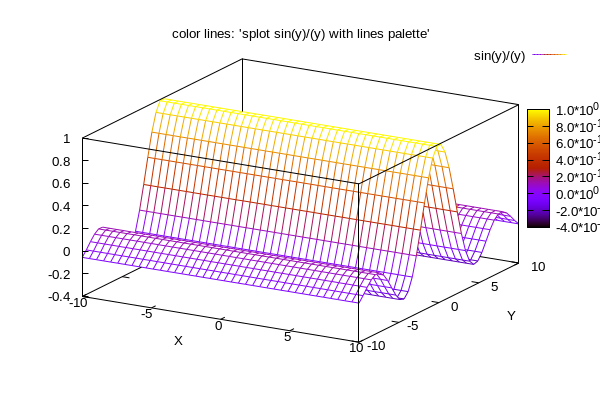
\includegraphics[width=0.5\textwidth]{supfig3}}
	\centering
	\caption{\textbf{\lipsum[30][5]} \lipsum[31][1-3]}
	\label{sup.fig:my_sup_plot3}
\end{figure}

\clearpage
\printbibliography[title=Supplementary References]

\end{document}
